
\documentclass[border=5pt]{standalone}
\usepackage{pgfplots}
\pgfplotsset{compat=1.18}
\begin{document}
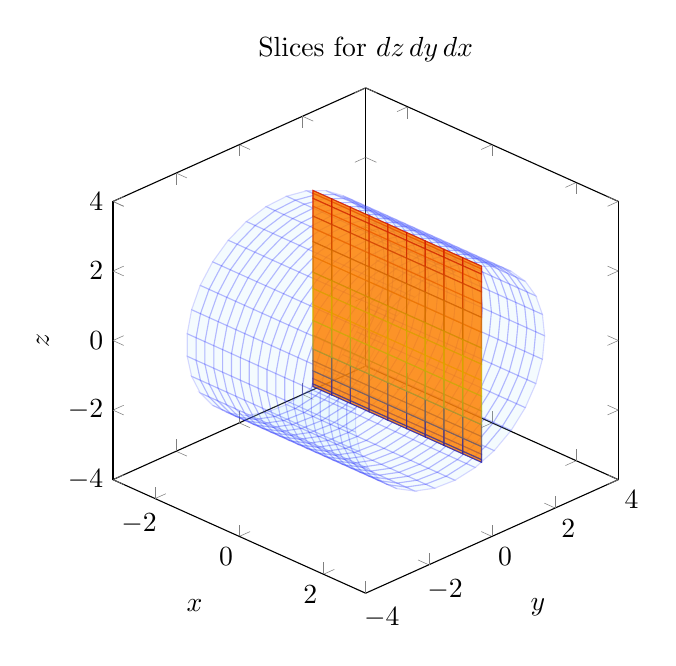
\begin{tikzpicture}
\begin{axis}[
    width=8cm, height=8cm,
    xlabel={$x$}, ylabel={$y$}, zlabel={$z$},
    xmin=-3, xmax=3, ymin=-4, ymax=4, zmin=-4, zmax=4,
    view={45}{30},
    title={Slices for $dz\,dy\,dx$},
]
% Cylinder
\addplot3[
    surf, opacity=0.15, fill=cyan!30, faceted color=blue,
    domain=-2:2, y domain=0:2*pi, samples=20, samples y=30,
] (x, {3*cos(deg(y))}, {3*sin(deg(y))});
% Highlight slice at y=1
\addplot3[
    surf, opacity=0.6, fill=orange,
    domain=-2:2, y domain=0:2*pi, samples=10, samples y=20,
] (x, 1, {sqrt(8)*sin(deg(y))});
\end{axis}
\end{tikzpicture}
\hspace{1em}
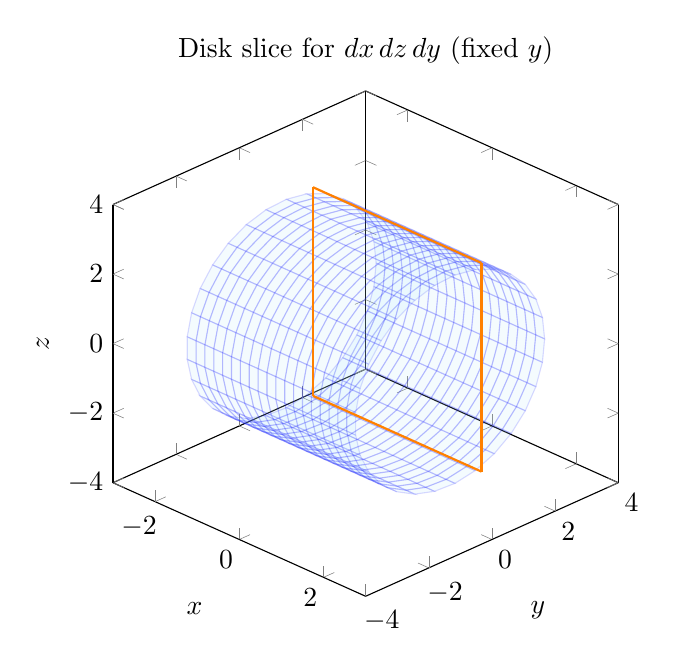
\begin{tikzpicture}
\begin{axis}[
    width=8cm, height=8cm,
    xlabel={$x$}, ylabel={$y$}, zlabel={$z$},
    xmin=-3, xmax=3, ymin=-4, ymax=4, zmin=-4, zmax=4,
    view={45}{30},
    title={Disk slice for $dx\,dz\,dy$ (fixed $y$)},
]
% Cylinder
\addplot3[
    surf, opacity=0.15, fill=cyan!30, faceted color=blue,
    domain=-2:2, y domain=0:2*pi, samples=20, samples y=30,
] (x, {3*cos(deg(y))}, {3*sin(deg(y))});
% Edges of highlighted disk slice at y=1
\addplot3[orange, thick, samples=50, domain=0:2*pi] (-2, 1, {3*sin(deg(x))});
\addplot3[orange, thick, samples=50, domain=0:2*pi] (2, 1, {3*sin(deg(x))});
\addplot3[orange, thick] coordinates {(-2,1,-3) (-2,1,3)};
\addplot3[orange, thick] coordinates {(2,1,-3) (2,1,3)};
\addplot3[orange, thick] coordinates {(-2,1,3) (2,1,3)};
\addplot3[orange, thick] coordinates {(-2,1,-3) (2,1,-3)};
\end{axis}
\end{tikzpicture}
\end{document}
